% Diese Datei ist Teil des Buchs "Schreibe Dein Programm!"
% Das Buch ist lizensiert unter der Creative-Commons-Lizenz
% "Namensnennung - Weitergabe unter gleichen Bedingungen 4.0 International (CC BY-SA 4.0)"
% https://creativecommons.org/licenses/by-sa/4.0/deed.de

\chapter{Gemischte Daten}
\label{cha:gemischte-daten}

Manchmal kommen an einer Stelle in unserem Problem verschiedene
Klassen der gleichen Sorte Daten vor:
%
\begin{itemize}
\item Ein Tier kann ein Gürteltier oder ein Papagei sein.
\item Eine Koordinate kann eine kartesische Koordinate oder eine
  Polarkoordinate sein.
\item Ein Essen kann ein Frühstück, Mittagessen oder Abendessen sein.
\end{itemize}
%
Solche Daten sind heißen \textit{gemischte Daten\index{gemischte
    Daten}}, und es handelt sich um eine weitere Form von
Falluntscheidungen, neben den aus Kapitel~\ref{cha:conditionals}
bekannten Aufzählungen und Zahlenbereichen.

Obwohl die Daten verschiedenartig sind, unterstützen sie doch
gemeinsame Operationen: Das Gewicht eines Tiers kann sowohl für
Gürteltiere als auch Papageien berechnet werden, der Abstand vom
Ursprung kann für beide Koordinatendarstellungen berechnet werden, die
Anzahl der Gänge kann für jede Art Essen bestimmt werden.

\section{Gemischte Daten}
\label{sec:mixed-data}
\label{sec:animal}

In der Einleitung war die Rede von Papageien:\index{Papagei} die benutzen wir, um
gemischte Daten einzuführen.  Vorher müssen wir jedoch Papageien mit den bekannten
Mitteln definieren.  Wir erweitern dafür die Datei mit dem Gürteltier
aus dem vorigen Kapitel.

Genau wie bei Gürteltieren interessiert uns bei Papageien das Gewicht,
aber wir nehmen an, da Papageien in der Regel nicht auf texanischen
Highways überfahren werden, dass sie immer lebendig sind.  Außerdem
betrachten wir ausschließlich sprechende Papageien, die jeweils einen
einzelnen Satz sagen können.  Hier die Datendefinition:
%
\begin{lstlisting}
; Ein Papagei hat folgende Eigenschaften:
; - Gewicht in Gramm
; - Satz, den er sagt
\end{lstlisting}
%
Hier die dazu passende Record-Definition:
%
\begin{lstlisting}
(define-record-functions parrot
  make-parrot
  (parrot-weight   natural)
  (parrot-sentence string))
\end{lstlisting}
%
\ldots{} und die passenden Signaturen:
%
\begin{lstlisting}
(: make-parrot (natural string -> parrot))
(: parrot-weight (parrot -> natural))
(: parrot-sentence (parrot -> string))
\end{lstlisting}
%
Hier zwei Beispiele für Papageien mit Kommentaren, die die Beziehung
zwischen Daten und Information beschreiben:
%
\begin{lstlisting}
(define parrot1 (make-parrot 10000 "Der Gärtner war's.")) ; 10kg, Miss Marple
(define parrot2 (make-parrot 5000 "Ich liebe Dich.")) ; 5kg, Romantiker 
\end{lstlisting}
%
Wir können einen Papagei ähnlich wie ein Gürteltier füttern~-- nur die
Portion ist kleiner, wir nehmen 50~g an.  Kurzbeschreibung und Signatur:\index{feed-parrot@\texttt{feed-parrot}}
%
\begin{lstlisting}
; Papagei mit 50 g Futter füttern
(: feed-parrot (parrot -> parrot))
\end{lstlisting}
%
Testfälle:
%
\begin{lstlisting}
(check-expect (feed-parrot parrot1) (make-parrot 10050 "Der Gärtner war's."))
(check-expect (feed-parrot parrot2) (make-parrot 5050 "Ich liebe Dich."))
\end{lstlisting}
%
Gerüst:
%
\begin{lstlisting}
(define feed-parrot
  (lambda (parrot)
    ...))
\end{lstlisting}
%
Die Schablone entsteht aus der Kombination der Schablonen für
zusammengesetzte Daten
als Einage (Konstruktionsanleitung~\ref{ka:zusammengesetzt-eingabe-schablone} auf
Seite \pageref{ka:zusammengesetzt-eingabe-schablone}) und als Ausgabe
(Konstruktionsanleitung~\ref{ka:zusammengesetzt-ausgabe-schablone} auf
Seite \pageref{ka:zusammengesetzt-ausgabe-schablone}):
%
\begin{lstlisting}
(define feed-parrot
  (lambda (parrot)
    (make-parrot ... ...)
    ... (parrot-weight parrot) ...
    ... (parrot-sentence parrot) ...))
\end{lstlisting}
%
\ldots{} und schließlich der vollständige Rumpf:
%
\begin{lstlisting}
(define feed-parrot
  (lambda (parrot)
    (make-parrot (+ (parrot-weight parrot) 50)
                 (parrot-sentence parrot))))
\end{lstlisting}
%
Fertig!

Du kannst Dir vielleicht vorstellen, dass Papageien und
Gürteltiere sich in einem Programm begegnen, also \emph{gemischt}
vorkommen.  Papageien und Gürteltiere gehören zum gemeinsamen
Oberbegriff \textit{Tier}\index{Tier}.  Dafür könnte eine
Beschreibung so aussehen:

\medskip

\noindent Ein \textit{Tier} ist eins der folgenden:
% 
\begin{itemize}
\item ein Gürteltier
\item ein Papagei
\end{itemize}
%
Die Formulierung "<eins der folgenden"> ist Dir schon aus
Abschnitt~\ref{sec:datendefinition} und
Konstruktionsanleitung~\ref{ka:fallunterscheidung} auf
Seite~\pageref{ka:fallunterscheidung} bekannt: Sie deutet auf eine
Fallunterscheidung\index{Fallunterscheidung} hin.

Da aber Gürteltiere und Papageien nicht als nur jeweils ein Wert
repräsentiert sind, handelt es sich nicht um eine Aufzählung: Die
beiden Fälle der Fallunterscheidung beschreiben unterschiedliche
\textit{Klassen}\index{Klasse} von Tieren, jede mit ihrer eigenen
Signatur.  Damit liegt eine neue Organisation von Daten vor:
\textit{gemischte Daten}.\index{gemischte Daten} Entsprechend ist es
durchaus sinnvoll, nach dem "<Gewicht eines Tiers"> zu fragen oder
"<ein Tier zu füttern">, was wir im folgenden auch vorhaben.

Die Beschreibung des Begriffs "<Tier"> ist bereits als Datendefinition
geeignet, und muss für Inklusion im Programm nur als Kommentar
umformatiert werden:
%
\begin{lstlisting}
; Ein Tier ist eins der folgenden:
; - Gürteltier
; - Papagei
\end{lstlisting}
%
Bei zusammengesetzen Daten kann die Datendefinition in eine
Record-Definition überführt werden.  In diesem Fall ist für jede
einzelne Klasse
Tier jeweils schon eine Record-Definition da.  Wenn wir Tiere im
allgemeinen in
Funktionen verarbeiten wollen, brauchen wir allerdings eine Signatur
für Tiere.  Zum Beispiel wollen wir eine Funktion schreiben, die für jedes
Tier das Gewicht ermittelt.  Diese Funktion könnte folgende Signatur haben:
%
\begin{lstlisting}
(: animal-weight (animal -> natural))
\end{lstlisting}
%%% HK: das \textbf war wohl ein Irrtum?
Wir brauchen also eine Definition für die Signatur \lstinline{animal}.
Diese sieht folgendermaßen aus:
%
\begin{lstlisting}
(define animal
  (signature
    (mixed dillo parrot)))
\end{lstlisting}
%
Das \lstinline{signature} kennen wir von den Fallunterscheidungen aus
Abschnitt~\ref{page:signature} auf Seite~\pageref{page:signature}.
Das \lstinline{mixed}\index{mixed@\texttt{mixed}} ist neu und steht
für "<gemischte Daten">, also Fallunterscheidungen, bei denen jeder
Fall seine eigene Signatur hat.  Du kannst die obige Definition lesen als
"<Tiere sind gemischt aus Gürteltieren und Papageien">; das klingt
aber auf Deutsch hölzern, weshalb wir für die Datendefinition bei der
Formulierung "<eins der folgenden"> bleiben.  Mit der Definition steht
die Signatur \lstinline{animal} zur Verfügung.  Wir haben schon mit der
Signatur für \lstinline{animal-weight} vorgegriffen.  Hier ist sie noch
einmal zusammen mit einer Kurzbeschreibung:
%
\begin{lstlisting}
; Gewicht eines Tiers feststellen
(: animal-weight (animal -> natural))
\end{lstlisting}
%
Diese Funktion sollte entsprechend für Gürteltiere \emph{und}
Papageien funktionieren, wir brauchen also Testfälle für beide:
%
\begin{lstlisting}
(check-expect (animal-weight dillo1) 55000)
(check-expect (animal-weight dillo2) 58000)
(check-expect (animal-weight parrot1) 10000)
(check-expect (animal-weight parrot2) 5000)
\end{lstlisting}
%
Das Gerüst sieht so aus:
%
\begin{lstlisting}
(define animal-weight
  (lambda (animal)
    ...))
\end{lstlisting}
%
Tiere bilden auch eine Fallunterscheidung in den Daten, mit zwei
Fällen: Gürteltiere und Papageien.  Im Rumpf der Funktion brauchen wir
also eine Verzweigung mit zwei Zweigen:
%
\begin{lstlisting}
(define animal-weight
  (lambda (animal)
    (cond
      (... ...)
      (... ...))))
\end{lstlisting}
%
Wir brauchen als nächstes zwei Bedingungen~-- eine, die Gürteltiere
und eine, die Papageien identifiziert.  Dafür erweitern wir die
Record-Definitionen um ein neues Element, das \textit{Prädikat}\index{Prädikat}.
Die Prädikate werden uns erlauben, die Bedingungen zu
schreiben.  Die Record-Definitionen sehen dann so aus:
%
\begin{lstlisting}
(define-record-functions dillo
  make-dillo
  dillo? ; |\(\Longleftarrow\)| Prädikat
  (dillo-weight natural)
  (dillo-alive? boolean))

(define-record-functions parrot
  make-parrot
  parrot? ; |\(\Longleftarrow\)| Prädikat
  (parrot-weight   natural)
  (parrot-sentence string))
\end{lstlisting}
%
Es sind zwei neue Namen hinzugekommen, \lstinline{dillo?} und
\lstinline{parrot?}. Das sind die Prädikate, und sie haben folgenden
Signaturen:
%
\begin{lstlisting}
(: dillo? (any -> boolean))
(: parrot? (any -> boolean))
\end{lstlisting}
%
Das \lstinline{any} ist auch neu und ist die Signatur für einen
beliebigen Wert: Ein Prädikat kann also auf absolut alles angewendet
werden.  Die beiden Prädikate unterscheiden Gürteltiere
beziehungsweise Papageien von anderen Werten:
%
\begin{lstlisting}
(dillo? dillo1)
|\evalsto| #t
(dillo? parrot1)
|\evalsto| #f
(parrot? dillo1)
|\evalsto| #f
(parrot? parrot1)
|\evalsto| #t
(dillo? 5)
|\evalsto| #f
(parrot? "foo")
|\evalsto| #f
\end{lstlisting}
%
Die Prädikate können wir benutzen, um die Bedingungen aus der
Schablone zu bestücken:
%
\begin{lstlisting}
(define animal-weight
  (lambda (animal)
    (cond
      ((dillo? animal) ...)
      ((parrot? animal) ...))))
\end{lstlisting}
%
Im ersten Zweig~-- dem Zweig für Gürteltiere~-- kommt nun
\lstinline{dillo-weight} zum Einsatz, im zweiten Zweig~-- für
Papageien~-- ist \lstinline{parrot-weight} zuständig:
%
\begin{lstlisting}
(define animal-weight
  (lambda (animal)
    (cond
      ((dillo? animal) (dillo-weight animal))
      ((parrot? animal) (parrot-weight animal)))))
\end{lstlisting}
% 
Fertig!

\begin{feature}{\texttt{define-record-functions} (mit Prädikaten)}{scheme:define-record-functions-predicates}
Eine \texttt{define"=record"=functions}"=Form\index{define-record-functions@\texttt{define-record-functions}}
hat folgende allgemeine Gestalt:
%
\begin{lstlisting}
(define-record-functions |\(t\)|
  |\(c\)|
  |\(p\)|
  (|\(\mathit{sel}\sb{1}\)| |\(\mathit{sig}\sb{1}\)|)
  |\(\ldots\)|
  (|\(\mathit{sel}\sb{n}\)| |\(\mathit{sig}\sb{n}\)|))
\end{lstlisting}
%
Diese Form definiert einen Record-Typ mit $n$ Feldern.
Dabei sind $t$, $c$, $\mathit{sel}_1 \ldots \mathit{sel}_n$ allesamt Variablen, für die
\lstinline{define-record-functions} Definitionen anlegt:
%
\begin{itemize}
\item $t$ ist der Name der Record-Signatur.
\item $c$ ist der Name des Konstruktors mit 
  folgender Signatur:
%  
\begin{lstlisting}
(: |\(c\)| (|\(\mathit{sig}\sb{1}\)| |\(\ldots\)| |\(\mathit{sig}\sb{n}\)| -> |\(t\)|))
\end{lstlisting}
\item $p$ ist der Name des Prädikats, der Records diesen Typs von
  anderen Werten unterscheidet.  Das Prädikat kann auch weggelassen
  werden.

    Das Prädikat hat folgende Signatur:
\begin{lstlisting}
(: |\(p\)| (any -> boolean))
\end{lstlisting}
\item $\mathit{Sel}_1, \ldots, \mathit{sel}_n$ sind die Namen der Selektoren für die Felder
  des Record-Typs.  Der Selektor $\mathit{sel}_i$ hat folgende Signatur:
% 
\begin{lstlisting}
(: |\(\mathit{sel}\sb{i}\)| (|\(t\)| -> |\(\mathit{sig}\sb{i}\)|))
\end{lstlisting}
\end{itemize}
%
\end{feature}
%
Abbildung~\ref{scheme:define-record-functions-predicates} ist eine
aktualisierte Beschreibung der Form von
\lstinline{define-record-functions}, bei der auch Prädikate
berücksichtigt sind

Aus diesem Beispiel ergibt sich eine Konstruktionsanleitung für
gemischte Daten.  Zunächst die Datenanalyse:

\begin{konstruktionsanleitung}{Gemischte Daten: Datenanalyse}
  \label{ka:gemischt-datenanalyse}
  Gemischte Daten sind Fallunterscheidungen, bei denen jeder Fall eine
  eigene Klasse von Daten mit eigener Signatur ist.
  Schreibe bei gemischten Daten eine Signaturdefinition der folgenden Form unter die
  Datendefinition:
%
\begin{lstlisting}
(define |\(\mathit{sig}\)|
  (signature
    (mixed |\(\mathit{sig}\sb{1}\)| |\(\mathit{sig}\sb{2}\)| |\(\ldots\)| |\(\mathit{sig}\sb{n}\)|)))
\end{lstlisting}
$\mathit{Sig}$ ist die Signatur für die neue Datensorte; $\mathit{sig}_1$ bis $\textit{sig}_n$
sind die Signaturen, aus denen die neue
Datensorte zusammengemischt ist.
\end{konstruktionsanleitung}
%
\noindent Die Konstruktionsanleitung für die Schablone ist der aus
der Konstruktionsanleitung~\ref{ka:fallunterscheidung-schablone} für
Fallunterscheidungen auf
Seite~\pageref{ka:fallunterscheidung-schablone} ähnlich:
%
\begin{konstruktionsanleitung}{Gemischte Daten als Eingabe:
    Schablone}
  \label{ka:gemischt-eingabe-schablone}
Eine Schablone für eine Funktion und deren Testfälle, die gemischte
Daten akzeptiert, kannst Du folgendermaßen konstruieren:
%
\begin{itemize}
\item Schreibe Tests für jeden der Fälle.
\item  Schreibe eine \lstinline{cond}-Verzweigung als Rumpf in die
  Schablone, die genau $n$ Zweige hat~-- also genau soviele Zweige,
  wie es Fälle in der Datendefinition beziehungsweise der Signatur gibt.
\item Schreibe für jeden Zweig eine Bedingung, der den entsprechenden
  Fall identifiziert.
\item Vervollständige die Zweige, indem Du eine Datenanalyse für
  jeden einzelnen Fall vornimmst und entsprechende Hilfsfunktionen
  und Konstruktionsanleitungen benutzt.
  Die übersichtlichsten Programme entstehen meist, wenn für jeden Fall
  separate Hilfsfunktionen definiert sind.\label{page:separate-mixed-procs}
\end{itemize}
%
\end{konstruktionsanleitung}
%
Eine Konstruktionsanleitung oder Schablone für gemischte Daten
\emph{als Ausgabe} ist unnötig~-- Du benutzt einfach die Schablone
des entsprechenden Falls.

Beachte den Unterschied zwischen \lstinline{enum} und
\lstinline{mixed}, die leicht zu verwechseln sind: \lstinline{One-of} steht
für "<einer der folgenden \emph{Werte}">, während \lstinline{mixed} für
"<gehörend zu einer der folgenden \emph{Signaturen}"> steht.

\begin{aufgabe}
  Denk Dir sinnvolle Datendefinitionen für Frühstück, Mittagessen und
  Abendessen aus (ein \ldots{}essen besteht aus \ldots), so dass es
  Sinn ergibt, für jede Sorte Essen die Frage "<Was für ein Gemüse ist
  enthalten?"> zu stellen.  Schreibe zunächst für jede Sorte Essen
  eine Funktion, die das enthaltene Gemüse liefert.  Schreibe dann
  eine Datendefinition für den Oberbegriff "<Essen">; ein Essen kann
  ein Frühstück, ein Mittagessen oder ein Abendessen sein.  Schreibe
  eine Funktion, welche das enthaltene Gemüse für ein Essen liefert.
\end{aufgabe}

\section{Die Lebensmittelampel}

In diesem Abschnitt nehmen wir uns noch ein weiteres Beispiel für
gemischte Daten vor, diesmal von vorneherein unter Benutzung der
Konstruktionsanleitung aus dem vorigen Abschnitt.

Die Lebensmittelampel ist eine Kennzeichnung auf Lebensmittelverpackungen,
die den Gehalt von gesundsheitsrelevanten Nährstoffen in den
Ampfelfarben ausweist: Grün für niedrigen Gehalt, Gelb für mittleren Gehalt und
Rot für hohen Gehalt. Bei Zucker zum Beispiel sieht die Ampel so aus, bezogen
auf 100~g eines Lebensmittels:
%
\begin{center}
  \begin{tabular}{l|l|l}
    grün & niedriger Gehalt &  weniger als 5 g\\
    gelb & mittlerer Gehalt & zwischen 5 g und 22,5 g\\
    rot & hoher Gehalt & mehr als 22,5 g
  \end{tabular}
\end{center}
%
Trotz der Bemühungen der Europäischen Union sind die
Bezeichnungen uneinheitlich.  Technisch gesehen ist die Ampel
redundant, wenn der Zuckergehalt in Gramm angegeben ist.
Manchmal ist allerdings der Zuckergehalt auch separat für Fruktose und
Glukose angegeben.

Ein Computerprogramm könnte aber den Umgang erleichtern, indem es jede
Angabe auf einer Lebensmittelpackung~-- Zucker in Gramm insgesamt,
Fruktose und Glukose separat sowie die Ampel~-- in die einheitliche
Ampel-Form bringt.  Schreiben wir also ein solches Programm.  Zunächst
die Datenanalyse:
%
\begin{itemize}
\item Die Zuckermenge in Gramm ist eine (rationale) Zahl.
\item Zuckeranteile bestehen aus der Menge von Fruktose und Glukose.
\item Eine Zuckerampel ist rot, gelb oder grün.
\item Der Zuckergehalt kann entweder als Zuckermenge, Zuckeranteile
  oder Zuckerampel angegeben werden.
\end{itemize}
%
Hier ist die Datendefinition für die zusammengesetzen Zuckeranteile:
%
\begin{lstlisting}
; Zuckeranteile bestehen aus:
; - Fruktose-Menge (in g)
; - Glukose-Menge (in g)
\end{lstlisting}
%
Daraus ergibt sich direkt die Record-Definition mit zwei Komponenten,
jeweils rationale Zahlen:
%
\begin{lstlisting}
(define-record-functions sugars
  make-sugars
  sugars?
  (sugars-fructose-g rational)
  (sugars-glucose-g  rational))
\end{lstlisting}
%
Hier einige Beispiele, zusammen mit Kommentaren, die die Beziehung
zwischen Daten und Information beschreiben:
%
\begin{lstlisting}
(define s1 (make-sugars 1 1)) ; 1 g Fruktose, 1 g Glukose
(define s2 (make-sugars 2 3)) ; 2 g Fruktose, 3 g Glukose
(define s3 (make-sugars 5 5)) ; 5 g Fruktose, 5 g Glukose
(define s4 (make-sugars 10 2.5)) ; 10 g Fruktose, 2.5 g Glukose
(define s5 (make-sugars 10 13)) ; 10 g Fruktose, 13 g Glukose
(define s6 (make-sugars 15 10)) ; 15 g Fruktose, 10 g Glukose
\end{lstlisting}
%
Bei der Ampel selbst handelt es sich um eine einfache
Fallunterscheidung:
%
\begin{lstlisting}
; Eine Ampel ist einer der folgenden Werte:
; - rot
; - gelb
; - grün
\end{lstlisting}
%
Das ist eine Aufzählung, wir geben entsprechend der dazu passenden
Signatur einen Namen:
%
\begin{lstlisting}
(define traffic-light
  (signature
   (enum "red" "yellow" "green")))
\end{lstlisting}
%
Die Angabe über den Zuckergehalt kann jede der drei oben genannten Formen
annehmen:
%
\begin{lstlisting}
; Ein Zuckergehalt ist eins der folgenden:
; - Gewicht in Gramm
; - Zuckeranteile
; - Ampelbezeichnung
\end{lstlisting}
%
Wieder ist an der Formulierung erkennbar, dass es sich um gemischte
Daten handelt, und zwar mit drei Fällen.  Das übersetzen wir in ein
Signaturdefinition mit \lstinline{mixed} und ebenfalls drei Fällen:
%
\begin{lstlisting}
(define sugar-content
  (signature
   (mixed rational
          sugars
          traffic-light)))
\end{lstlisting}
%
Das Beispiel zeigt, dass die Fälle einer Definition für gemischte Daten
nicht allesamt Records sein müssen.  Es ist allerdings wichtig, dass
die Fälle \emph{disjunkt} sind, also jeder Wert eindeutig einem der
Fälle zugeordnet werden kann: Sonst wäre es nicht möglich, eine sinnvolle
Verzweigung zu schreiben, welche die Fälle unterscheidet.

Nun zu unserer Funktion zur Ermittlung der Ampelbezeichnung für den
Zuckergehalt.  Hier Kurzbeschreibung und Signatur:
%
\begin{lstlisting}
; Ampelbezeichnung für Zuckergehalt ermitteln
(: sugar-traffic-light (sugar-content -> traffic-light))
\end{lstlisting}
%
Wir brauchen ziemlich viele Testfälle, um alle Fälle von
Zuckergehalt abzudecken sowie die Eckfälle der Tabelle von oben.
%
\begin{lstlisting}
(check-expect (sugar-traffic-light 2) "green")
(check-expect (sugar-traffic-light 5) "yellow")
(check-expect (sugar-traffic-light 10) "yellow")
(check-expect (sugar-traffic-light 12.5) "yellow")
(check-expect (sugar-traffic-light 23) "red")

(check-expect (sugar-traffic-light s1) "green")
(check-expect (sugar-traffic-light s2) "yellow")
(check-expect (sugar-traffic-light s3) "yellow")
(check-expect (sugar-traffic-light s4) "yellow")
(check-expect (sugar-traffic-light s5) "red")
(check-expect (sugar-traffic-light s6) "red")

(check-expect (sugar-traffic-light "green") "green")
(check-expect (sugar-traffic-light "yellow") "yellow")
(check-expect (sugar-traffic-light "red") "red")
\end{lstlisting}
%
Als nächstes ist, wie immer, das Gerüst dran:
%
\begin{lstlisting}
(define sugar-traffic-light
  (lambda (sugar-content)
    ...))
\end{lstlisting}         
%
Als nächstes wenden wir die Schablone für Funktionen an, die gemischte
Daten akzeptieren.  Wir brauchen eine Verzweigung mit sovielen Zweigen
wie \lstinline{sugar-content} Fälle hat, also drei:
%
\begin{lstlisting}
(define sugar-traffic-light
  (lambda (sugar-content)
    (cond
      (... ...)
      (... ...)
      (... ...))))
\end{lstlisting}         
%
Als nächstes brauchen wir Tests für die drei Fälle.  Für den zweiten
Fall ist das einfach, da es sich um \lstinline{sugars}-Records handelt:
da gibt es das Prädikat \lstinline{sugars?}.  Beim ersten Fall handelt es
sich aber um eine rationale Zahl, beim dritten um eine Zeichenkette~--
beides eingebaute Datensorten.  Für diese gibt es die eingebauten
Prädikate \lstinline{rational?} und \lstinline{string?}~--
Abbildung~\ref{scheme:predicates} zählt noch mehr eingebaute
Prädikate auf.
%
\begin{feature}{Eingebaute Prädikate}{scheme:predicates}
  \index{Prädikate|eingebaut}\index{eingebaute Prädikate}
  Folgende Prädikate sind eingebaut:
  \begin{itemize}
  \item \lstinline{number?}\index{number?@\texttt{number?}} testet, ob ein Wert eine Zahl ist.
  \item \lstinline{real?}\index{real?@\texttt{real?}} testet, ob ein Wert eine reelle Zahl ist.
  \item \lstinline{rational?}\index{rational?@\texttt{rational?}} testet, ob ein Wert eine rationale Zahl ist.
  \item \lstinline{natural?}\index{natural?@\texttt{natural?}} testet, ob ein Wert eine natürliche Zahl ist.
  \item \lstinline{string?}\index{string?@\texttt{string?}} testet, ob ein Wert eine Zeichenkette ist.
  \item \lstinline{boolean?}\index{boolean?@\texttt{boolean?}} testet, ob ein Wert ein boolescher Wert ist.
  \end{itemize}
\end{feature}
%
Mit dieser Information gewappnet können wir die Tests ergänzen:
%
\begin{lstlisting}
(define sugar-traffic-light
  (lambda (sugar-content)
    (cond
      ((rational? sugar-content) ...)
      ((sugars? sugar-content) ...)
      ((string? sugar-content) ...))))
\end{lstlisting}         
%
Im ersten Zweig handelt es sich nicht nur um eine rationale Zahl,
sondern auch um eine Fallunterscheidung mit drei Fällen entsprechend
der Tabelle vom Anfang:
%
\begin{lstlisting}
(define sugar-traffic-light
  (lambda (sugar-content)
    (cond
      ((rational? sugar-content) 
       (cond
         (... ...)
         (... ...)
         (... ...)))
      ((sugars? sugar-content) ...)
      ((string? sugar-content) ...))))
\end{lstlisting}         
%
Als nächstes ergänzen wir Tests entsprechend der Tabelle:
%
\begin{lstlisting}
(define sugar-traffic-light
  (lambda (sugar-content)
    (cond
      ((rational? sugar-content) 
       (cond
         ((< sugar-content 5) ...)
         ((and (>= sugar-content 5) (<= sugar-content 12.5)) ...)
         ((> sugar-content 12.5) ...)))
      ((sugars? sugar-content) ...)
      ((string? sugar-content) ...))))
\end{lstlisting}         
%
Schließlich müssen wir noch die Antworten eintragen:
%
\begin{lstlisting}
(define sugar-traffic-light
  (lambda (sugar-content)
    (cond
      ((rational? sugar-content) 
       (cond
         ((< sugar-content 5) "green")
         ((and (>= sugar-content 5) (<= sugar-content 12.5)) "yellow")
         ((> sugar-content 12.5) "red")))
      ((sugars? sugar-content) ...)
      ((string? sugar-content) ...))))
\end{lstlisting}         
%
Das verschachtelte \lstinline{cond} ist etwas unübersichtlich: In
Konstruktionsanleitung~\ref{ka:gemischt-eingabe-schablone} auf
Seite~\pageref{page:separate-mixed-procs} ist bereits vermerkt, dass
es sinnvoll ist, diesen Zweig in eine separate Hilfsfunktion
auszulagern.  Hier sind Kurzbeschreibung und Signatur für diese
Hilfsfunktion:
%
\begin{lstlisting}
; Zuckeranteil in g in Ampel umwandeln
(: sugar-weight->traffic-light (rational -> traffic-light))
\end{lstlisting}
%
Die Testfälle lassen sich aus den Testfällen für
\lstinline{sugar-traffic-light} durch einfaches Kopieren und Umbenennen
gewinnen:
%
\begin{lstlisting}
(check-expect (sugar-weight->traffic-light 2) "green")
(check-expect (sugar-weight->traffic-light 5) "yellow")
(check-expect (sugar-weight->traffic-light 10) "yellow")
(check-expect (sugar-weight->traffic-light 12.5) "yellow")
(check-expect (sugar-weight->traffic-light 23) "red")
\end{lstlisting}
%
Gerüst:
%
\begin{lstlisting}
(define sugar-weight->traffic-light
  (lambda (sugar-weight)
    ...))
\end{lstlisting}
%
Den Rumpf haben wir ja schon geschrieben, wir müssen ihn nur noch
hierher bewegen und \lstinline{sugar-content} in \lstinline{sugar-weight} umbenennen. Das \drscheme{}-System
bietet dazu nach einem Klick auf "<Syntaxprüfung"> die Möglichkeit, mit einem
Rechtsklick auf den Parameter \lstinline{sugar-content} ein Menü aufzuklappen, das unter
anderem die Auswahl "<\lstinline{sugar-content} umbenennen"> anbietet. \drscheme{} sorgt dann
dafür, dass alle zugehörigen Vorkommen von \lstinline{sugar-content} in gleicher Weise
umbenannt werden.\label{def:sugar-weight-traffic-light}
%
\begin{lstlisting}
(define sugar-weight->traffic-light
  (lambda (sugar-weight)
    (cond
      ((< sugar-weight 5) "green")
      ((and (>= sugar-weight 5) (<= sugar-weight 22.5)) "yellow")
      ((> sugar-weight 12.5) "red"))))
\end{lstlisting}
%
Zurück zu \lstinline{sugar-traffic-light}: Dort benutzen wir zunächst die
neu definierte Hilfsfunktion:
%
\begin{lstlisting}
(define sugar-traffic-light
  (lambda (sugar-content)
    (cond
      ((rational? sugar-content)
       (sugar-weight->traffic-light sugar-content))
      ((sugars? sugar-content) ...)
      ((string? sugar-content) ...))))
\end{lstlisting}         
%
Beim nächsten Zweig geht es um den Fall \lstinline{sugars}~--
zusammengesetzte Daten.  Wir können also die entsprechende Schablone
anwenden:
%
\begin{lstlisting}
(define sugar-traffic-light
  (lambda (sugar-content)
    (cond
      ((rational? sugar-content)
       (sugar-weight->traffic-light sugar-content))
      ((sugars? sugar-content) ... (sugars-fructose-g sugar-content) ...
                   ... (sugars-glucose-g sugar-content) ...)
      ((string? sugar-content) ...))))
\end{lstlisting}         
%
Wir müssen Fruktose- und den Glukose-Anteil addieren und die Summe
dann ebenfalls entsprechend der Tabelle vom Anfang in eine Ampelfarbe
umwandeln.  Aber halt!~-- Genau für das Umwandeln der Zahl aus der
Tabelle in eine Ampelfarbe haben wir ja gerade die Hilfsfunktion
\lstinline{sugar"=weight->traffic"=light} geschrieben, und diese
können wir %%HK 2020-01-27: "= funktioniert im lstinline nicht!
erneut zum Einsatz bringen:
%
\begin{lstlisting}
(define sugar-traffic-light
  (lambda (sugar-content)
    (cond
      ((rational? sugar-content)
       (sugar-weight->traffic-light sugar-content))
      ((sugars? sugar-content)
       (sugar-weight->traffic-light (+ (sugars-fructose-g sugar-content)
                                       (sugars-glucose-g sugar-content))))
      ((string? sugar-content) ...))))
\end{lstlisting}         
%
Bleibt der letzte Fall~-- der ist zum Glück trivial, da es sich schon
um eine Farbe handelt, Die muss \lstinline{sugar-traffic-light} nur
zurückgeben:
%
\begin{lstlisting}
(define sugar-traffic-light
  (lambda (sugar-content)
    (cond
      ((rational? sugar-content)
       (sugar-weight->traffic-light sugar-content))
      ((sugars? sugar-content)
       (sugar-weight->traffic-light (+ (sugars-fructose-g sugar-content)
                                       (sugars-glucose-g sugar-content))))
      ((string? sugar-content) sugar-content))))
\end{lstlisting}         
%
Fertig!

\section{Fehler repräsentieren}
\label{sec:slope}
\label{sec:maybe}

Dieser Abschnitt beschreibt eine weitere häufig vorkommende Anwendung
für gemischte Daten.  Es geht um Situationen, wo eine Funktion
keine sinnvolle Antwort weiß.

Als Beispiel schreiben wir eine Funktion, welche die Steigung einer
Geraden auf der Ebene berechnet anhand der Koordinaten zweier Punkte
darauf.  Die Funktion akzeptiert vier Argumente: Die X- und die Y-Koordinate des
ersten Punkts und danach die X- und die Y-Koordinate des zweiten
Punkts.  Wir fangen mit Kurzbeschreibung, Signatur, einigen Tests
und einem Gerüst an:
%
\begin{lstlisting}
; Steigung einer Gerade berechnen
(: slope (real real real real -> real))

(check-expect (slope 0 0 1 1) 1)
(check-expect (slope 0 0 2 1) 1/2)
(check-expect (slope 1 2 3 5) 3/2)

(define slope
  (lambda (x1 y1 x2 y2)
    ...))
\end{lstlisting}
%
Die Formelsammlung sagt, dass wir zur Berechnung der Steigung die
Differenz der Y-Koordinaten durch die Differenz der X-Koordinaten
teilen müssen:
%
\begin{lstlisting}
(define slope
  (lambda (x1 y1 x2 y2)
    (/ (- y2 y1)
       (- x2 x1))))
\end{lstlisting}
%
Fertig, könnte man meinen.  Es gibt aber Linien, die keine Steigung
haben.  In der REPL sieht das so aus:
%
\begin{alltt}
> (slope 0 0 0 1)
{\color{red}/: durch 0 geteilt}
\end{alltt}
%
Die Meldung ist ein bisschen unfreundlich und birgt mehrere Probleme:
%
\begin{itemize}
\item Die Meldung besagt zwar, was das Programm gemacht hat (durch 0
  geteilt), aber benennt nicht die Ursache des Problems: dass die
  Gerade keine Steigung hat.
\item Das Programm bricht einfach ab, ohne dass es eine Möglichkeit
  bekommt, mit dem Problem umzugehen.
\item Dass das Programm einfach abbrechen kann, ist aus der Signatur
  nicht ersichtlich, die suggeriert, dass die Funktion immer eine
  reelle Zahl zurückliefert.
\end{itemize}
%
Alle drei Probleme können wir auf einmal mit gemischten Daten lösen.
Dazu müssen wir zunächst dafür sorgen, dass die Funktion einen
sinnvollen Wert zurückliefert, bevor sie durch 0 teilen würde.
Dadurch werden die Eingaben in zwei Klassen aufgeteilt: Es gibt eine
Steigung oder eben nicht.  Es bietet sich eine binäre Verzweigung an,
um diese beiden Klassen zu unterscheiden:
%
\begin{lstlisting}
(define slope
  (lambda (x1 y1 x2 y2)
    (if (= (- x2 x1) 0)
        ...
        (/ (- y2 y1)
           (- x2 x1))))) 
\end{lstlisting}
%
Nur müssen wir anstelle der Ellipse irgendetwas ins Programm
schreiben.  Wir können nicht einfach irgendeine reelle Zahl nehmen, da
diese ja auch eine legitime Steigung sein könnte.  Stattdessen
brauchen wir einen Wert, den wir von den legitimen Zahlen
unterscheiden können.  Wir könnten eine spezielle Zeichenkette oder
\lstinline{#f} benutzen.  (Siehe dazu Aufgabe~\ref{aufgabe:no-slope}
auf Seite~\pageref{aufgabe:no-slope}.)

Wir empfehlen aber, stattdessen einen eigenen Record-Typ zu
definieren, und zwar so:
%
\begin{lstlisting}
; Es gibt keine Steigung
(define-record-functions no-slope
  make-no-slope
  no-slope?)
\end{lstlisting}
%
Dieser Record-Typ hat keine Felder, das heißt, er kann nur benutzt
werden, um einen einzigen Wert herzustellen, nämlich
\lstinline{(make-no-slope)}.  (Es handelt sich also um eine
degenerierte Version von zusammengesetzten Daten ohne Bestandteile.)
Diesen Wert können wir aber durch das Prädikat \lstinline{no-slope?}
von allen anderen Werten unterscheiden und benutzen ihn, wenn es keine
Steigung gibt:
%
\begin{lstlisting}
(define slope
  (lambda (x1 y1 x2 y2)
    (if (= (- x2 x1) 0)
        (make-no-slope)
        (/ (- y2 y1)
           (- x2 x1)))))
\end{lstlisting}
%
Jetzt können wir einen Testfall definieren:
%
\begin{lstlisting}
(check-expect (no-slope? (slope 0 0 0 1)) #t)
\end{lstlisting}
%
Allerdings liefert \drscheme{} für diesen Testfall eine
Signaturverletzung: Die Signatur tut ja immer noch so, als würde immer
eine reelle Zahl herauskommen.  Wir erweitern sie also folgendermaßen:
%
\begin{lstlisting}
(: slope (real real real real -> (mixed real no-slope)))
\end{lstlisting}
%
Dieser Signatur sieht man unmittelbar an, was sie liefert und kann aus
den Namen auch schließen, was die beiden Fälle bedeuten.  Natürlich
könnten wir eine eigene Signatur definieren wie sonst bei gemischten
Daten, das lohnt aber hier kaum.

\section*{Aufgaben}

\begin{aufgabe}
  Vereinfache in der Funktion \lstinline{sugar-weight->traffic-light} auf
  Seite~\pageref{def:sugar-weight-traffic-light} die Bedingungen, wie
  in Abschnitt~\ref{page:bedingungen-vereinfachen} auf
  Seite~\pageref{page:bedingungen-vereinfachen} beschrieben.
\end{aufgabe}

\begin{aufgabe}
  Ein Supermarkt möchte seine Waren in einem Programm verwalten. Es gibt
  drei Warenklassen:
  \begin{description}
  \item[Essen] beschrieben durch einen Namen, den Stückpreis, das Mindesthaltbarkeitsdatum
    und den aktuellen Bestand im Supermarkt
  \item[Getränke] beschrieben durch einen Namen, den Stückpreis, das Mindesthaltbarkeitsdatum
    und den Bestand. Zusätzlich muss hier noch festgehalten werden, ob Pfand verlangt wird.
  \item[Sonstige] beschrieben durch einen Namen, den Stückpreis und den Bestand.
  \end{description}

  
  \begin{enumerate}
  \item Führe eine Datenanalyse durch und erstelle Daten- und 
    Record-Definitionen.
  \item Schreibe eine Funktion \lstinline{stückpreis}, die eine Warenklasse
    akzeptiert und den Stückpreis zurückgibt.
  \item Schreibe eine Funktion \lstinline{buchen}, die eine Warenklasse und die Anzahl der
    abzubuchenden Exemplare akzeptiert, den Bestand der Warenklasse reduziert und die
    Warenklasse zurückgibt. Falls mehr Exemplare gefordert werden, als in der Warenklasse
    vorhanden sind, soll der Bestand auf 0 gesetzt werden.
  \item Schreibe eine Funktion \lstinline{haltbar?}, die eine
    Warenklasse und ein Datum akzeptiert und \lstinline{#t} zurückgibt, falls das
    Mindesthaltbarkeitsdatum (MHD) nicht überschritten wurde. Falls kein MHD bekannt ist,
    soll \lstinline{#t} zurückgeben werden.
  \end{enumerate}
\end{aufgabe}

\begin{aufgabe}
  \label{aufgabe:knaubichler2}
  Erweitere die Lösung von Aufgabe~\ref{aufgabe:knaubichler} aus
  dem vorigen Kapitel (Seite~\pageref{aufgabe:knaubichler}):
  
  \begin{enumerate}
  \item Schreibe nun eine Funktion, die zwei
    Grundkreaturen in beliebiger Reihenfolge akzeptiert, die Kreuzung
    vornimmt und eine neue Kreatur zurückgibt.
    
  \item Schreibe nun eine
    Funktion, die drei Grundkreaturen in beliebiger Reihenfolge
    akzeptiert, die Kreuzung vornimmt und eine neue Kreatur
    zurückgibt.
  \end{enumerate}
\end{aufgabe}     

\begin{aufgabe}

  Das Spiele-Entwicklungsteam von
  \textit{Exciting Games, Inc.} ist in Personalnot: Für die
  Implementierung des bahnbrechenden 2D-Spiels \textit{The Adventures
    of DrRacket} wird dringend eine Repräsentation der grafischen
  Formen Kreis, Rechteck und Dreieck benötigt.  Alle Hacker
  sind leider wahnsinnig damit beschäftigt, bunte Pixel in der Gegend
  herumzuschieben und können sich daher nicht dieser grundlegenden
  Aufgabe widmen.  Deswegen fällt Dir diese Aufgabe zu!  Dir geht
  nur ein mit Pizzabelag verschmierter Zettel zu, der offenbar als
  Arbeitsanweisung gedacht ist.  Darauf steht:
  \begin{itemize}

  \item Es gibt drei Klassen von Formen: Kreise, Rechtecke und
    gleichschenklige Dreiecke.  Alle Formen haben eine
    Ursprungskoordinate und enthalten eine Information über die Größe
    (Radius, Höhe, Breite, etc), wie Du auf der Abbildung siehst.
    Benutze für die Ursprungskoordinate die vorgegebenen kartesischen
    Koordinaten!

    % \begin{figure}[h]
    \begin{center}
      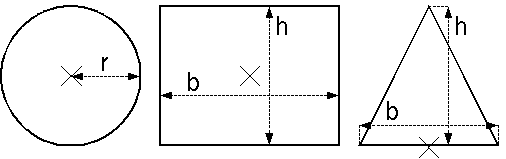
\includegraphics[height=1.8cm]{i1gem/shapes.png}
      % \caption{Formen}
      % \label{Formen}
    \end{center}
    % \end{figure}

  \item Es soll Funktionen geben, die auf allen Formen funktionieren
    und Folgendes leisten:

    \begin{itemize}

    \item kartesische Koordinate einer Form zurückgeben

    \item $x$-Koordinate einer Form zurückgeben

    \item $y$-Koordinate einer Form zurückgeben

    \item Abstand des Ursprungs einer Form zum Ursprung des
      Koordinatensystems zurückgeben

    \item Flächeninhalt einer Form zurückgeben

    \item Form um $\Delta_x$ in $x$-Richtung und um $\Delta_y$ in
      $y$-Richtung verschieben, also eine Form zurückgeben, deren
      Ursprungskoordinate entsprechend verschoben ist

%     \item Größe einer Form um einen Faktor ändern, also eine Form
%       zurückgeben, deren Größe entsprechend angepasst ist
  \item  Flächeninhalt zweier
    Formen vergleichen: Für gleich große Formen liefert die Funktion
    \verb|"equal"| zurück, sonst \verb|"smaller"|, wenn die erste
    Form kleiner ist, beziehungsweise \verb|"bigger"|, wenn die erste
    Form größer ist.
    \end{itemize}

  \end{itemize}
  %
  Zeige den Hackern, was richtiges Software-Engineering ist und
  benutze die passenden Konstruktionsanleitungen, um Repräsentationen für die Formen und die zugehörigen
  Funktionen zu schreiben!
\end{aufgabe}

\begin{aufgabe}

  Es gibt verschiedene Verstöße gegen die
  Straßenverkehrsordnung: 
  \begin{itemize}
  \item Falschparken mit Ort und Zeitpunkt des Verstoßes

  \item Überfahren einer roten Ampel mit Ort und Zeitpunkt des Verstoßes
    sowie der Dauer in Sekunden, wie lange die Ampel bereits rot war

  \item Überhöhte Geschwindigkeit mit Ort und Zeitpunkt des Verstoßes
    sowie der Höhe der Geschwindigkeits"-über"-tre"-tung
  \end{itemize}
  Neben den angegebenen Bestandteilen muss später für jeden Verstoß vermerkt 
  werden, ob zusätzlich eine "<Gefährdung des Straßenverkehrs"> vorliegt.
  
  \begin{enumerate}
  \item Schreibe eine Datendefinition für
    Verstöße gegen die Straßenverkehrsordnung.  Schreibe Daten-
    und Record-Definitionen für die verschiedenen Verstöße.  
    Die Zeitpunkte kannst Du durch Zeichenketten wie \verb|"11.4.1971 22:00"| repräsentieren.  
    Gib alle Signaturen an!

  \item Schreibe eine Funktion, die einen
    beliebigen Verstoß entgegennimmt und den Ort des Verstoßes
    zurückgibt.

    Schreibe analog eine Funktion, die einen
    beliebigen Verstoß entgegennimmt und den Zeitpunkt des Verstoßes
    zurückgibt.

  \item Schreibe eine Funktion, die einen
    beliebigen Verstoß entgegennimmt, diesen als Gefährdung des
    Straßenverkehrs betrachtet und wieder zurückgibt (das heißt jeder 
    Verstoß ist ein Verstoß mit Gefährdung).
  \end{enumerate}

  Die Verstöße haben unterschiedliche Tatbestände zur Folge:

  \begin{itemize}
  \item Einfaches Vergehen mit Bußgeld

  \item Ordnungswidrigkeit mit Bußgeld, Punkte für die
    Verkehrssünderdatei und Fahrverbot in Monaten

  \item Straftat mit Punkten für die Verkehrssünderdatei und
    Freiheitsstrafe in Monaten
  \end{itemize}
  
  \begin{enumerate} \setcounter{enumii}{3}
  \item Schreibe eine Datendefinition für
    Tatbestände auf Verstöße gegen die Straßenverkehrsordnung.
    Schreibe Daten- und Record-Definitionen für die verschiedenen
    Tatbestände.  Gib alle Signaturen an!

  \item Schreibe eine Funktion, die einen
    beliebigen Tatbestand akzeptiert und die Anzahl der anfallenden
    Punkte zurückliefert.
  \end{enumerate}

  Schreibe nun Funktionen, die Verstöße akzeptieren und die
  Tatbestände berechnen:

  \begin{enumerate} \setcounter{enumii}{5}
  \item Schreibe eine Funktion, die Falschparken
    akzeptiert und ein einfaches Vergehen mit 20~Euro Bußgeld zurückgibt.
    Wenn das Falschparken eine Gefährdung des Straßenverkehrs
    darstellt (z.B.  bei Behinderung von Rettungsfahrzeugen),
    soll die Funktion eine Ordnungswidrigkeit mit 40~Euro Bußgeld,
    einem Punkt und keinem Fahrverbot zurückgeben.

  \item Schreibe eine Funktion, die Überfahren
    einer roten Ampel akzeptiert und eine Ordnungswidrigkeit
    zurückgibt.  Dabei gilt:
    \begin{itemize}
    \item wenn die Ampel kürzer als eine Sekunde rot war und keine
      Gefährdung vorlag: 50~Euro, 3~Punkte, kein Fahrverbot
    \item wenn die Ampel mindestens eine Sekunde rot war oder eine
      Gefährdung vorlag: 125~Euro, 4~Punkte, 1~Monat Fahrverbot
    \end{itemize}

  \item Schreibe eine Funktion, die überhöhte
    Geschwindigkeit akzeptiert und den Tatbestand zurückgibt.  Dabei
    gilt:
    \begin{itemize}
    \item Geschwindigkeitsübertretung weniger als 20 km/h ohne Gefährdung:
      einfaches Vergehen mit 35~Euro
    \item Geschwindigkeitsübertretung zwischen 20 und 40 km/h
      (inklusive) ohne Gefährdung: Ordnungswidrigkeit mit 75~Euro,
      3~Punkten und 1~Monat Fahrverbot
    \item Geschwindigkeitsübertretung von mehr als 40 km/h ohne
      Gefährdung: Ordnungswidrigkeit mit 200~Euro, 4~Punkte und
      3~Monate Fahrverbot
    \item bei gleichzeitiger Gefährdung des Straßenverkehrs: Straftat
      mit 3~Punkte mehr als ohne Gefährdung angegeben und
      Freiheitsstrafe, die doppelt so lang ist wie das Fahrverbot, das
      ohne Gefährdung gilt (wenn es kein Fahrverbot gibt, dann gibt es
      auch keine Freiheitsstrafe)
    \end{itemize}

  \item Schreibe eine Funktion, die einen
    Verstoß akzeptiert und dessen Folge zurückgibt.  Benutze die
    Funktionen aus den vorherigen Teilaufgaben.
  \end{enumerate}
\end{aufgabe}

\begin{aufgabe}\label{aufgabe:no-slope}
  Experimentiere für die Funktion \lstinline{slope} in
  Abschnitt~\ref{sec:slope} auf Seite~\pageref{sec:slope}
  mit anderen Repräsentationen als einem eigenen
  Record-Typ für "<keine Steigung">:
  %
  \begin{itemize}
  \item Liefere \lstinline{#f} zurück.
  \item Liefere eine Zeichenkette \lstinline{"no slope"} zurück.
  \end{itemize}
  %
  Wie muss jeweils die Signatur von \lstinline{slope} lauten?
  
  Wie könnte ein Programm dann nach einem Aufruf feststellen, ob es
  keine Steigung gab?  Schreibe für beide Varianten ein Prädikat
  \lstinline{no-slope?} diese Situation feststellt.

  Was haben die insgesamt drei Varianten für die Repräsentation von
  "<keine Steigung"> jeweils für Vor- und Nachteile?
\end{aufgabe}

%%% Local Variables: 
%%% mode: latex
%%% TeX-master: "i1"
%%% End: 
